\chapter{Resultados}
	\section{Introducción} 
	
	Este capítulo presenta los resultados obtenidos durante la implementación de cada uno de los prototipos planteados en el Capítulo
	~\ref{chap:disenoeimpl} y durante la ejección de los casos de prueba correspondientes. 
	
	Para la ejecución de todas las pruebas se utilizó la placa desarrollo S3ADSP1800A del fabricante Xilinx que cumple con los requerimientos detallados
	en la Tabla ~\ref{tab:requsr1} y se encontraba dentro de las alternativas disponibles al momento del desarrollo de este trabajo. Aún cumpliendo con
	los requerimientos especificados, la placa de desarrollo no cuenta con un completo soporte de periféricos on board ni con amplia documentación de
	apoyo respecto de la materia. Se presentaron grandes dificultades en el acceso a la memoria SPI FLASH S33 de Intel la cual se encuentra soportada por
	herramientas \textit{oficiales} que únicamente corren bajo Windows. Alternativamente existe una versión de la placa de desarrollo S3ADSP1800A,
	disponible también en el laboratorio del CUDAR, que se encuentra equipada con una memoria FLASH SPI Numonyx M25P64 que puede ser accedida mediante
	herramientas de programación como XC3SPROG y UrJTAG alojando finalmente los programas necesarios para el arranque del sistema.
	
	Las pruebas realizadas con el sistema operativo de tiempo real ecOS proveyeron información útil para el desarrollo de sistemas embebidos de tiempo
	real. Se analizaron inicialmente las capacidades y limitaciones en la ejecución de hilos. Aunque estas pruebas tan solo verifican la utilización de
	una parte las capacidades, el sistema operativo ecOS posee mayor funcionalidad que no fue probada en este trabajo y presenta capacidades comparables
	a implementaciones como lo son FreeRTOS y su implentación comercial eCosPro.
	
	La capacidad, por defecto, del Kernel de Linux de ser compilado para arquitecturas OpenRISC posibilitó tener un entorno de ejecución de amplia
	funcionalidad y gran utilización en el ámbito de desarrollo de Sistemas Embebidos.  
	
	\newpage
	\section{Resultados de Utilización de FPGA en la Implementación del Proyecto MinSoC}

	A continuación se presentan los resultados obtenidos luego del proceso completo de implementación del proyecto.  Los resultados de la herramienta PAR
	se muestran en la referencia ~\ref{lst:resultparminsoc}

\begin{lstlisting}[frame=single,caption={Resumen de utilización - MinSoC},label={lst:resultparminsoc},breaklines]

Logic Utilization:
 Number of Slice Flip Flops:         5,040 out of  33,280   15%
 Number of 4 input LUTs:            13,901 out of  33,280   41%

Logic Distribution:
 Number of occupied Slices:          8,475 out of  16,640   50%
   Number of Slices containing only related logic:   8,475 out of   8,475 100%
   Number of Slices containing unrelated logic:          0 out of   8,475   0%
     *See NOTES below for an explanation of the effects of unrelated logic.
 Total Number of 4 input LUTs:      14,231 out of  33,280   42%
   Number used as logic:            13,866
   Number used as a route-thru:        330
   Number used for Dual Port RAMs:      32
     (Two LUTs used per Dual Port RAM)
   Number used as Shift registers:       3

 The Slice Logic Distribution report is not meaningful if the design is
 over-mapped for a non-slice resource or if Placement fails.

 Number of bonded IOBs:                 29 out of     519    5%
 Number of BUFGMUXs:                     5 out of      24   20%
 Number of DCMs:                         1 out of       8   12%
 Number of BSCANs:                       1 out of       1  100%
 Number of DSP48As:                      4 out of      84    4%
 Number of RAMB16BWERs:                 70 out of      84   83%
 Number of BSCAN_SPARTAN3As:             1 out of       1  100%

Average Fanout of Non-Clock Nets:                3.74

\end{lstlisting}

	El proyecto MinSoC se encuentra enfocado a su utilización en sistemas embebidos de capacidades ajustadas sintetizables en una gran cantidad de FPGA
	de diversos desarrolladores. La facilidad de adaptación del proyecto para ser portado a otras arquitecturas reconfigurables le confiere gran
	versatilidad ampliando notablemente su gama de aplicación.
	Durante el desarrollo de las pruebas se prentendió esteblecer los límites de aplicación del proyecto que establezcan referencias sólidas para una
	futura elección del proyecto en aplicaciones reales.

\newpage
\section {Estudio de Capacidades del Proyecto MinSoC}
		\subsection{Resultados de la ejecución del multiplicador de matrices binarias}
		Se presentan a continuación los resultados de ejecución del programa multiplicador de matrices binarias. Se utilizó un gráfico que muestra el orden
		de las matrices multiplicadas vs. la cantidad de ticks de ejecución. El gráfico ~\ref{fig:mulmat} muestra con claridad que el tiempo de ejecución
		aumenta exponencialmente a medida que aumenta el orden de las matrices multiplicadas.  
		
\begin{figure}[h!]
 	\begin{center}
  	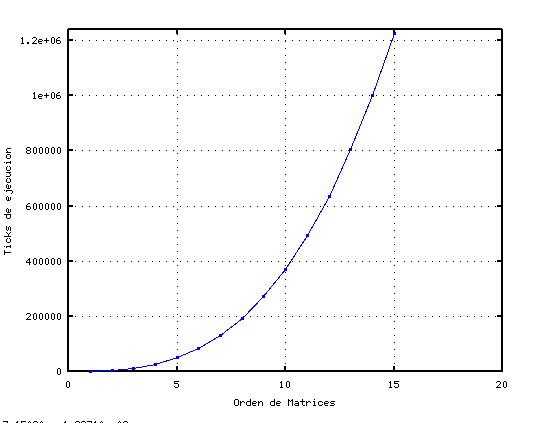
\includegraphics[width=0.6\textwidth,keepaspectratio=true]{./images/matrices}
  	\caption{Multiplicación de matrices binarias}
  	\label{fig:mulmat}
 	\end{center}
	\end{figure}

		Teniendo en cuenta que la aplicación fue ejecutada en una versión sintentizada básica del proyecto minSoC, este no posee unidades de multiplicación
		por hardware que efectuen cálculos con mayor eficiencia, reduciendo el tiempo de ejecución. Pueden considerarse también, las optimizaciones del
		compilador pero este aspecto fue analizado en el Prototipo Tres con mayor detalle. 
		
\newpage
	\section{Resultados de Utilización de FPGA en la Implementación del Proyecto ORPSoC}
	
	A continuación se presentan los resultados obtenidos luego del proceso completo de implementación del proyecto.  Los resultados de la herramienta PAR
	se muestran en la referencia ~\ref{lst:resultorpsoc}
		
\begin{lstlisting}[frame=single,caption={Resumen de utilización - ORPSoC},label={lst:resultorpsoc},breaklines]

Device utilization summary:

Selected Device : 3sd1800afg676-4 

Number of Slices:                     6696  out of  16640    40%  
Number of Slice Flip Flops:           4872  out of  33280    14%  
Number of 4 input LUTs:              12093  out of  33280    36%  
   Number used as logic:             11009
   Number used as Shift registers:     124
   Number used as RAMs:                960
Number of IOs:                         128
Number of bonded IOBs:                 128  out of    519    24%  
   IOB Flip Flops:                       7
Number of BRAMs:                        14  out of     84    16%  
Number of GCLKs:                         8  out of     24    33%  
Number of DCMs:                          2  out of      8    25%  
Number of DSP48s:                        4  out of     84     4%  

Partition Resource Summary:

No Partitions were found in this design.
\end{lstlisting}	
		
		\subsection{Place and route}	
		
		Los resultados de la herramienta de place and route se pueden encontrar en el archivo de registros <orpsoc.par>. Este archivo contiene información
		respecto de la cantidad de bloques de entrada y salida internos, externos y la cantidad de otros componentes lógicos utilizados. 
		
\begin{lstlisting}[frame=single,caption={Resultado de PAR - ORPSoC},label={lst:salidas},breaklines]
Design Summary Report:
 Number of External IOBs                         128 out of 519    24%
   Number of External Input IOBs                 21
      Number of External Input IBUFs             21

   Number of External Output IOBs                44
      Number of External Output DIFFMLRs          2
      Number of External Output DIFFSLRs          2
      Number of External Output IOBs             14
      Number of External Output IOBLRs           26

   Number of External Bidir IOBs                 63
      Number of External Bidir DIFFMLRs           4
      Number of External Bidir DIFFSLRs           4
      Number of External Bidir IOBs              22
      Number of External Bidir IOBLRs            33

   Number of BUFGMUXs                        7 out of 24     29%
   Number of DCMs                            2 out of 8      25%
   Number of DSP48As                         4 out of 84      4%
   Number of RAMB16BWERs                    16 out of 84     19%
   Number of Slices                       7772 out of 16640  46%
    Number of SLICEMs                      612 out of 8320    7%
\end{lstlisting}

		\subsection{Reporte de timing}	

El reporte de timing presenta los resultados del análisis de distribución de los clocks del proyecto. Entre los resultados se obtiene el mínimo
periodo (Máx Frecuencia) necesarios para el correcto funcionamiento del sistema. Es importante destacar que los tiempos expuestos en el reporte son
teóricos y se presentan cambios importante durante las pruebas sobre el hardware. 

\begin{lstlisting}[frame=single,caption={Reporte timing - ORPSoC},label={lst:salidas},breaklines]
Timing summary:

Timing errors: 498  Score: 729028  (Setup/Max: 311057, Hold: 417971)
Constraints cover 395663179 paths, 94 nets, and 53193 connections

Design statistics:
  Minimum period:  45.166ns   (Maximum frequency:  22.141MHz)
  Maximum path delay from/to any node:  11.696ns
  Maximum net delay:   2.594ns
  Minimum input required time before clock:  26.237ns
  Maximum output delay after clock:  13.126ns
\end{lstlisting}

		
\section {Estudio de Capacidades del Proyecto ORPSoC}	
		\subsection{Condiciones de entorno de ejecución para benchmark}
		
		En la siguente tabla~\ref{tab:conbench} se muestran las condiciones del entorno de prueba durante los benchmarks.  

		\begin{table}[h!]
		\begin{tabular}{ |p{5cm} |p{10cm}| }    
		\hline
		\multicolumn{2}{|>{\columncolor[gray]{.8}}c}{Condiciónes de entorno de prueba|}\\
		\hline
		Placa de desarrollo & S3ADSP1800A  \\
		\hline 
		FPGA & Xilinx Spartan-3 XC3SD1800A \\ 
		\hline 
		Reloj del procesador & 25 MHz\\ 
		\hline
		Caché de instrucciones  & 8 KB \\ 
		\hline
		Caché de datos	  & 8 KB\\ 
		\hline	
		MMU & Sí \\	
		\hline
		Multiplicador hardware & Sí \\		
		\hline	
		División hardware & Sí \\		
		\hline	
\end{tabular}
%\end{center}
\caption{Condiciones del entorno de prueba}
\label{tab:conbench}
\end{table}

				\subsection{Resultados de la ejecución del benchmark CoreMark}
		
Inicialmente se prensentan los valores obtenidos durante la ejecución del Benchmark compilado con optimizaciones de nivel 2 (-O2) del
compilador cruzado. El Benchmark CoreMark arroja un valor de  41.288895/25MHz = 1.65/MHz como resultado de la prueba. Las condiciones de ensayo se
detallaron en la tabla~\ref{tab:conbench} y la ejecución se realizó con 600 iteraciones. 


	\subsection {Presentación de los resultados de optimización} 
	
Aquí están los resultados obtenidos mediante la utilización de optimización en la fase de compilación. Al ser compilado con el nivel de optimización
-O2 y diferentes flags de optimización se observaron los resultados mostrados en el bloque ~\ref{lst:salidasO2}

\begin{lstlisting}[frame=single,caption={Optimización nivel -O2 - Flags activos : -FUNROLL-LOOPS },label={lst:salidasO2},breaklines]
2K validation run parameters for coremark.
CoreMark Size    : 666
Total ticks      : 1527
Total time (secs): 15.270000
Iterations/Sec   : 39.292731
Iterations       : 600
Compiler version : GCC4.5.1-or32-1.0rc4
Compiler flags   : -O2  -mboard=s3adsp1800a -FUNROLL-LOOPS -DVALIDATION_RUN=1  
\end{lstlisting}

\begin{lstlisting}[frame=single,caption={Optimización nivel -O2 - Flags activos : -MSOFT-FLOAT},label={lst:salidas},breaklines]
2K validation run parameters for coremark.
CoreMark Size    : 666
Total ticks      : 1528
Total time (secs): 15.280000
Iterations/Sec   : 39.267016
Iterations       : 600
Compiler version : GCC4.5.1-or32-1.0rc4
Compiler flags   : -O2  -mboard=s3adsp1800a -MSOFT-FLOAT -DVALIDATION_RUN=1  
\end{lstlisting}

\begin{lstlisting}[frame=single,caption={Optimización nivel -O2 - Flags activos : -FUNROLL-ALL-LOOPS},label={lst:salidas},breaklines]
2K validation run parameters for coremark.
CoreMark Size    : 666
Total ticks      : 1528
Total time (secs): 15.280000
Iterations/Sec   : 39.267016
Iterations       : 600
Compiler version : GCC4.5.1-or32-1.0rc4
Compiler flags   : -O2  -mboard=s3adsp1800a -FUNROLL-ALL-LOOPS -DVALIDATION_RUN=1  
\end{lstlisting}

\begin{lstlisting}[frame=single,caption={Optimización nivel -O2 - Flags activos : -FGCSE-SM},label={lst:salidas},breaklines]
2K validation run parameters for coremark.
CoreMark Size    : 666
Total ticks      : 1527
Total time (secs): 15.270000
Iterations/Sec   : 39.292731
Iterations       : 600
Compiler version : GCC4.5.1-or32-1.0rc4
Compiler flags   : -O2  -mboard=s3adsp1800a -FGCSE-SM -DVALIDATION_RUN=1  
\end{lstlisting}

\begin{lstlisting}[frame=single,caption={Optimización nivel -O3 - Sin Flags activos},label={lst:salidas},breaklines]
2K validation run parameters for coremark.
CoreMark Size    : 666
Total ticks      : 1654
Total time (secs): 16.540000
Iterations/Sec   : 36.275695
Iterations       : 600
Compiler version : GCC4.5.1-or32-1.0rc4
Compiler flags   : -O3  -mboard=s3adsp1800a -DVALIDATION_RUN=1  
\end{lstlisting}

\begin{lstlisting}[frame=single,caption={Optimización nivel -O3 - Flags activos -MHARD-DIV -MHARD-MULT},label={lst:salidas},breaklines]
2K validation run parameters for coremark.
CoreMark Size    : 666
Total ticks      : 1654
Total time (secs): 16.540000
Iterations/Sec   : 36.275695
Iterations       : 600
Compiler version : GCC4.5.1-or32-1.0rc4
Compiler flags   : -O3  -mboard=s3adsp1800a -MHARD-DIV -MHARD-MULT -DVALIDATION_RUN=1  
\end{lstlisting}

\begin{lstlisting}[frame=single,caption={Optimización nivel -O3 - Flags activos -FUNROLL-LOOPS},label={lst:salidas},breaklines]
2K validation run parameters for coremark.
CoreMark Size    : 666
Total ticks      : 1655
Total time (secs): 16.550000
Iterations/Sec   : 36.253776
Iterations       : 600
Compiler version : GCC4.5.1-or32-1.0rc4
Compiler flags   : -O3  -mboard=s3adsp1800a -FUNROLL-LOOPS -DVALIDATION_RUN=1  
\end{lstlisting}

\begin{lstlisting}[frame=single,caption={Optimización nivel -O3 - Flags activos -FGCSE-SM},label={lst:salidas},breaklines]
2K validation run parameters for coremark.
CoreMark Size    : 666
Total ticks      : 1654
Total time (secs): 16.540000
Iterations/Sec   : 36.275695
Iterations       : 600
Compiler version : GCC4.5.1-or32-1.0rc4
Compiler flags   : -O3  -mboard=s3adsp1800a -FGCSE-SM -DVALIDATION_RUN=1  
\end{lstlisting}

\begin{lstlisting}[frame=single,caption={Optimización nivel -O3 - Flags activos -MSOFT-FLOAT},label={lst:salidas},breaklines]
2K validation run parameters for coremark.
CoreMark Size    : 666
Total ticks      : 1655
Total time (secs): 16.550000
Iterations/Sec   : 36.253776
Iterations       : 600
Compiler version : GCC4.5.1-or32-1.0rc4
Compiler flags   : -O3  -mboard=s3adsp1800a -MSOFT-FLOAT -DVALIDATION_RUN=1  
\end{lstlisting}

\begin{lstlisting}[frame=single,caption={Optimización nivel -O3 - Flags activos -FUNROLL-ALL-LOOPS},label={lst:salidas},breaklines]
2K validation run parameters for coremark.
CoreMark Size    : 666
Total ticks      : 1654
Total time (secs): 16.540000
Iterations/Sec   : 36.275695
Iterations       : 600
Compiler version : GCC4.5.1-or32-1.0rc4
Compiler flags   : -O3  -mboard=s3adsp1800a -FUNROLL-ALL-LOOPS -DVALIDATION_RUN=1  
\end{lstlisting}

\begin{lstlisting}[frame=single,caption={Optimización nivel -O3 - Flags activos -FUNROLL-LOOPS -MSOFT-FLOAT
-FUNROLL-ALL-LOOPS -FGCSE-SM},label={lst:salidas},breaklines]
2K validation run parameters for coremark.
CoreMark Size    : 666
Total ticks      : 1654
Total time (secs): 16.540000
Iterations/Sec   : 36.275695
Iterations       : 600
Compiler version : GCC4.5.1-or32-1.0rc4
Compiler flags   : -O3  -mboard=s3adsp1800a -FUNROLL-LOOPS -MSOFT-FLOAT -FUNROLL-ALL-LOOPS -FGCSE-SM -DVALIDATION_RUN=1  
\end{lstlisting}


\begin{table}[h!]
\begin{center}
\begin{tabular}{ |l |l| l|}
\hline
\rowcolor[gray]{0.8} Opciones del compilador&-O2&-O3 \\
\hline
Sin extras 					&1.65 			&1.54\\
\hline
-mhard-div -mhard-mu 		& 1.57			&1.45\\
\hline
-funroll-loops			 	& 1.57			& 1.45 \\
\hline
-fgcse-sm					& 1.57			& 1.45\\
\hline
-msoft-float 				& 1.57			&1.45 \\
\hline
-funroll-all-loops	 		& 1.57			& 1.45 \\
\hline
Todos	 					& 1.57			& 1.45 \\
\hline
\end{tabular}
\end{center}
\caption{Compilación con distintos niveles y flags de optimización}
\end{table}

En la siguiente tabla ~\ref{tab:compcoremark} se presenta una comparativa con resultados Coremark de varios microprocesadores entre los que se
encuentran los microprocesadores softcore privativos de los principales Fabricantes.

\begin{table}[h!]
\begin{center}
\begin{tabular}{ |p{4cm} |p{4cm}|p{0.8cm}|p{1.5cm}|p{2.1cm}|p{2.2cm}|}
\hline
\rowcolor[gray]{0.8} Procesador &	Compilador &	 Mhz &	CoreMark / MHz &	Core Mark &	 Core Mark / Core \\
\hline
	Openrisc 1200 & or32-elf-gcc 4.5.1-or32.1.0rc4							&25		&1.45   &36.27		&36.27 \\
\hline
	Altera Nios II & nios2-elf-gcc.exe (Altera 12.1 Build 177) gcc 4.1.2	&200	&0.93 	&186.27 	&186.27\\
\hline
	Altera Nios II & nios2-elf-gcc.exe (Altera 12.1 Build 177) gcc 4.1.2	&200	&1.60 	&320.59 	&320.59\\
\hline
	ARM Cortex-A9  (Exynos4 Quad) &	armcc 5.03-24							&1400	&15.89 	&22243.00 	&5560.75\\
\hline
	ARM Cortex-A15 &	armcc 5.03-24											&1700	&9.36 	&15908.00 	&7954.00\\
\hline
	Xilinx XC7Z020 ARM Cortex-A9 MPcore &	GCC4.7.2							&800	&5.92 	&4737.47 	&2368.73\\
\hline
	Xilinx XC7Z7045 ARM Cortex-A9 MPcore&	GCC4.7.2						&1000	&5.93 	&5927.24 	&2963.62\\
\hline
	Xilinx XC7Z020 Dual Core ARM Cortex-A9 MPcore&	GCC4.6.1				&667	&3.38 	&2256.15 	&1128.07\\
\hline
	Xilinx MicroBlaze v8.20.b in Virtex5 FPGA, 5-stage pipeline, 16K/16K cache &	GCC4.1.2 20070214 (Xilinx 13.4 Build EDK\_O.87 25 Nov 2011)	
																			&125	&1.90   &238.00 	&238.00 \\
\hline
	Altera Nios II &	nios2-elf-gcc.exe (Altera 10.1 Build 153) 4.1.2			&80		&1.49 	&119.00		&119.00\\
\hline
	Xilinx MicroBlaze 7.10d in Virtex4-FX20 FPGA, 5-stage pipeline, 16K/16K cache&	GCC4.1.2 20070214 (Xilinx 12.3 Build EDK\_MS3.66 14 Jul 2010)	
																			&100	&1.75	&174.59 	&174.59\\
\hline
	ARMv7 Processor rev 3 (v7l) &	Android NDK-r5 (GCC 4.4.3)					&600	&2.04 	&1221.15	&1221.15\\ 
\hline
	ARM Cortex-A9 MPCore on FPGA &	GCC 4.3.3 (Sourcery G++ Lite 2009q1-203)		&1		&11.52 	&11.52 		&2.88 	 	\\
\hline
	ARM ARM1176JZ-S	on FPGA & GCC 4.3.3 (Sourcery G++ Lite 2009q1-203)				&1		&2.08 	&2.08 		&2.08		\\
\hline
\end{tabular}
\end{center}
\caption{Compartiva de resultados Coremark}
\label{tab:compcoremark}
\end{table}


\newpage

		\subsection{Resultados de la ejecución del benchmark Dhyrstone}
		
		Es un benchmark sintético y comercial. Intenta medir la velocidad del sistema en cuanto a rendimiento no numérico, expresando los
		resultados en DPS (instrucciones Dhrystones Por Segundo). El rendimiento de Dhyrstone se calcula a partir de la siguiente fórmula: Iteraciones
		Dhrystone por segundo = reloj del procesador * número de pasadas / tiempo de ejecución. Para que el resultado sea válido el código Dhrystone debe
		ser ejecutado al menos por dos segundos. Es un pequeño benchmark sintético que pretende ser representativo de programación entera de
		sistemas. 
		
		Contiene muchas instrucciones simples, llamadas a procedimiento y condicionales, y pocas de coma flotante y bucles. Usa pocas variables globales y
		ejecuta operaciones con punteros. Está compuesto por 12 procedimientos incluidos en un bucle de medida con 94 sentencias. No se puede variar su
		tamaño. Está compuesto por un 53\% de instrucciones de asignación, 32\% de instrucciones de control y un 15\% de llamadas a procedimiento.
		Dhrystone es compacto (no más de 1,5 KB), ampliamente disponible en el dominio público, y sencillo de ejecutar. Por ser tan pequeño el Dhrystone
		entra completamente en la caché interna, de esta manera no mide el resto del sistema pero presenta la ventaja de que mide solamente la capacidad
		del procesador para trabajar con enteros.

		En esta sección se muestran los resultados de la ejección del Benchmark Drystone. Inicialmente, se compiló la aplicación sin optimizaciones del
		compilador con 1.000.000 y 500.000 iteraciones del benchmark. Luego, se realizaron compilaciones con diferentes niveles y flags de optimización. 

		Los resultados obtenidos al ejecutar Dhrystone en sus diferentes construcciones se presenta en la Referencia~\ref{lst:Dhrystone}

\begin{lstlisting}[frame=single,caption={Sin optimizaciones },label={lst:Dhrystone},breaklines]

Execution starts, 1000000 runs through Dhrystone
Timer ticks, 100/s., (7397 - 0) =	7397
Number of Runs 1000000
Elapsed time 73.97s
Processor at 25 MHz
Microseconds for one run through Dhrystone: ( 73970000 uS / 1000k ) = 73 uS
Dhrystones per Second:                      13698 
\end{lstlisting}

\begin{lstlisting}[frame=single,caption={Optimización nivel -O2},label={lst:salidas},breaklines]
Execution starts, 500000 runs through Dhrystone
Timer ticks, 100/s., (3699 - 0) =	3699
Number of Runs 500000
Elapsed time 36.99s
Processor at 25 MHz
Microseconds for one run through Dhrystone: ( 36990000 uS / 500k ) = 73 uS
Dhrystones per Second:                      13888 
\end{lstlisting}

\begin{lstlisting}[frame=single,caption={Optimización nivel -O3},label={lst:salidas},breaklines]
Execution starts, 500000 runs through Dhrystone
Timer ticks, 100/s., (2738 - 0) =	2738
Number of Runs 500000
Elapsed time 27.38s
Processor at 25 MHz
Microseconds for one run through Dhrystone: ( 27380000 uS / 500k ) = 54 uS
Dhrystones per Second:                      18518 
\end{lstlisting}


	\subsection {Presentación de los resultados de optimización} 

El Dhrystone compara el rendimiento del procesador usando una máquina de referencia: la VAX 11/780 es la máquina que corre a 1 DMIP (logra 1757
Dhrystones por segundo). No se puede parametrizar, a diferencia del Whetstone donde los distintos tipos de instrucción están en bucles, aquí los
mismos no existen por lo que no se puede cambiar la importancia de cada tipo de instrucción alterando la cantidad de veces que se itera cada bucle.

En base a los resultados de ejecución se calcularon los siguientes 

\begin{table}[h!]
\begin{center}
\begin{tabular}{ |l |l |l |l |}
\hline
\rowcolor[gray]{0.8} Opciones del compilador& Sin Optimizaciones & -O2 &-O3 \\
\hline
DMIPS 					& 7.79 			&   7.90  &  10.53  \\
\hline
\end{tabular}
\end{center}
\caption{Comparación de compilación con distintos niveles de optimización}
\end{table}


En la siguiente tabla se presenta una comparativa con resultados Dhrystone de varios microprocesadores comerciales.

\begin{table}[h!]
\begin{center}
\begin{tabular}{ |l |l |l |l |}
\hline
\rowcolor[gray]{0.8} Microprocesador& MHz & DMIPS con Optimizaciones & DMIPS sin Optimizaciones \\
\hline
Openrisc		  &25	&10.53	&7.9\\
\hline
AMD 80386         &40   &17.5   &4.32\\
\hline
IBM 486D2         &50   &26.6   &7.89\\
\hline
80486 DX2         &66   &45.1   &12.0\\
\hline
IBM 486BL        &100   &53.9   &12.0\\
\hline
AMD 5X86         &133   &84.5   &9.37\\
\hline
Pentium           &75    &112   &19.3\\
\hline
Cyrix P150       &120    &175   &27.9\\
\hline
Pentium          &100    &169   &31.8\\
\hline
Cyrix PP166      &133    &219   &38.4\\
\hline
IBM 6x86         &150    &234   &44.1\\
\hline
Pentium          &133    &239   &38.3\\
\hline
\end{tabular}
\end{center}
\caption{Comparativa de resultados Dhrystone}
\end{table}

	%\section{Estudio de factibilidad para la implentación de RTOS Embebidos}
	%Durante las pruebas realizadas en el prototipo ~\ref{chap:proto4} 
	
	%\subsection{Resultados del programa de prueba de hilos}
	%\section{Estudio de factibilidad para la implentación Linux}
	
	
	 